\chapter{Diseño y Ensamblado}
\label{ch:DisenoEnsamblado}

En esta sección se describirán los pasos necesarios para la concreción física
del proyecto.
Se comenzará con la confección e interpretación del diagrama de cañerías e
instrumentación, con el objetivo de validar la solución propuesta en
\ref{sec:SolucionPropuesta}.
Luego se hará énfasis en la construcción de la planta a partir de los elementos
disponibles.
Se describirá en detalle cada uno de ellos y se hará mención de
las decisiones constructivas tomadas durante el ensamblado.

\section{P\&ID}
\label{sec:p&id}

\subsection{Diagrama de cañerías e instrumentación}
Un diagrama de cañerías e instrumentación es un esquema de la planta en donde
pueden observarse todos los elementos que componen el proceso.
Estos diagramas emplean símbolos para representar cada elemento y sus
conexiones.
Los elementos presentes en este esquema están regidos por la norma
\emph{Standard S5.1 Instrumentation Symbol Specification}.
\todo{poner norma en anexo}
El diagrama permite una rápida comprensión del proceso, y se denomina
corrientemente \gls{pyid}.

Cada elemento debe ir acompañado de una denominación, que utiliza la
siguiente codificación:

\begin{itemize}  
 \item \textbf{Primer letra:}
 designa la variable medida. Puede ser :
 \begin{itemize}
  \item Presión
  \item Nivel
  \item Caudal
  \item Temperatura
 \end{itemize}

 \item \textbf{Letras siguientes:}
 designa la función del componente, o modifica el sentido de la primer letra.
 Puede ser:
 \begin{itemize}
  \item Indicador
  \item Almacenaje de datos
  \item Controlador
  \item Transmisor
 \end{itemize}
\end{itemize}

\subsection{P\&ID de nuestra planta}
De acuerdo a los componentes detallados en la sección
\ref{sec:MaterialesDisponibles} se realizó el esquema \gls{pyid} de la planta
de control de nivel.
\todo{Lo dejamos a esto?}{\color{red} Se utilizó una plantilla disponible en
Google Docs, dado que era suficiente para la complejidad de nuestro proyecto.}
Para la correcta comprensión de este capítulo es indispensable contar con el
esquema, que puede encontrarse en el anexo \ref{anexo:pyid}.
\todo{Poner diag en anexo}

\section{Estructura de Soporte}
\label{sec:EstructuraSoporte}

Dado que el objetivo principal del proyecto es que la planta sirva para fines
educativos, se opta por utilizar una estructura móvil.
De esta manera, la posición de la planta puede modificarse según se requiera.

\todo{imagen de la estructura y medidas}
La estructura, de caño estructural, puede apreciarse en la figura x.
Está dotada de cuatro ruedas con frenos de seguridad, que permiten fijar la
planta al momento de una demostración.
Sus dimensiones se presentan en la tabla \ref{tab:dimensionesEstructura}.

\begin{table}
\centering
\begin{tabular}{|l|l|}
\hline
Alto & $\,m$\\
Ancho &  $\,m$\\
Profundidad &  $\,m$\\
\hline
\end{tabular}
\caption{Dimensiones de la estructura de soporte}
\label{tab:dimensionesEstructura}
\end{table}
 
La estructura presenta en su sección media barras de refuerzo.
Sobre ellas se colocaron los tanques.
Además, sobre las barras se fijó una base de madera, donde se coloca la
válvula electroneumática, las celdas de presión diferencial
y las bombas.
La manguera que corresponde al tiempo muerto se colocó bajo
las barras de refuerzo.
En la parte superior de la planta se instaló una pequeña base de
madera donde irá montado el receptor inalámbrico.
Ya está incluida en la estructura el tablero\todo{características}, donde se
montarán los elementos eléctricos y electrónicos.

Al comienzo del proyecto la estructura de caño estaba ya soldada y pintada, con
las ruedas colocadas.
No obstante, el grupo de trabajo tuvo que barnizar las maderas.

\section{Cañerías}
\label{sec:Canerias}

\subsection{Mangueras y Caños}
Luego de analizar el esquema \gls{pyid}, se observa que las cañerías deben
formar un circuito cerrado (\emph{loop}), diferenciando
claramente las cañerías de vaciado y llenado.
Las conexiones fueron echas mayormente en caño de polipropileno de 3/4
pulgadas.
En otros puntos del circuito, se optó por utilizar manguera de alta presión
telada de 3/4 pulgadas.
Las cañerías utilizadas son suficientes para las presiones de trabajo del
proyecto, del orden de \todo{Con que
presión trabaja la planta? 10 m para las bombas, verificar presión max de
caños}.

Teniendo los elementos montados sobre la planta (bombas, tanques, válvula
electroneumática) se decidió la manera de realizar el conexionado.
El caño rígido presenta la dificultad de no tener tolerancia al momento de
realizar uniones.
Además, para realizar tuberías complejas con muchas curvas, es necesario
colocar un gran número de componentes suplementarios (uniones dobles,
niples).
La cañería se torna compleja, dificultando la comprensión del circuito
hidráulico por parte del alumno.
Es por ello que se opto por usar en diferentes partes de la planta mangueras
flexibles:

\begin{itemize}
  \item \textbf{Salida del tanque de reserva - entrada a la bomba B1}:
  se utilizo manguera flexible dado que la estructura no permitía colocar caños
  rígidos: los elementos de polipropileno necesarios eran más grandes que el
  espacio disponible en la estructura.

  \item \textbf{Salida de la bomba B1 - entrada a la válvula:}
  se utilizo manguera, para evitar una unión doble en un trayecto muy pequeño.
  
  \item \textbf{Salida de la válvula - entrada al tanque controlado:}
  debido a la longitud del tramo se opto usar caños rígidos.
  Además, se montaron los elementos de medición sobre la cañería (manómetro y
  placa orificio).
  
  \item \textbf{Salida del tanque controlado - entrada a la bomba B2:}
  debido al mismo problema de falta de espacio, se opto por el uso de manguera
  flexible.
  
  \item \textbf{Salida de la bomba - entrada al tanque de reserva:}
  esta conexión es la más larga y en ella van montados manómetros y
  válvulas manuales. Por ello, se eligió una cañería rígida de polipropileno.

  \item \textbf{Conexión de perturbación de las bombas:}
  se utilizó manguera flexible, para evitar uniones dobles y
  niples que requieren de una gran precisión durante el montaje.
 \end{itemize}

Por ultimo se procedió a pintar los caños mediante un código de colores.
 \begin{itemize}
  \item {\color{Cerulean} \textbf{Celeste:}} llenado del tanque controlado.
  \item {\color{YellowOrange} \textbf{Amarillo:}} vaciado del tanque controlado.
 \end{itemize}
El código de colores, si bien no es estándar en la industria, permite una fácil
comprensión del circuito hidráulico.
\todo{bella imagen de los colores de la cañería}

\subsection{Tiempo Muerto}
\label{subsec:tiempoMuerto}
Se colocó en la planta un circuito de tiempo muerto, que consta de 20 \todo{no
son 30?} metros de manguera negra de 1/2 pulgada.
El tiempo muerto se coloca en paralelo de la cañería de llenado (ver
\gls{pyid}).
Mediante una válvula manual puede elegirse utilizar o no el tiempo muerto.

El objetivo del tiempo muerto es alejar la acción de control del tanque
controlado.
El sensor de nivel tardará un tiempo adicional $t_d$ en observar los cambios
que se producen en la válvula electroneumática \cite{bib:ApuntesPuglesiTema2}.
La función de transferencia de la planta cambiará notablemente:
\begin{itemize}
 \item Por un lado, el retraso en la respuesta debe ser tenido en cuenta
 \begin{align}
  G_{td}(s) &= e^{-t_d\,s}\,G(s)
 \end{align}
 donde $G(s)$ corresponde a la función de transferencia de una planta sin
 tiempo muerto, y $G_{td}(s)$ es la misma planta con tiempo muerto.
  \item Por otro lado, se agregan pérdidas por rozamiento del
  fluido cambiando la función de transferencia original $G(s)$ de nuestra
  planta.
\end{itemize}
En conclusión, el proceso a controlar es diferente comparado con proceso sin
tiempo muerto.
La inclusión esta cañería adicional permite disponer de dos escenarios
diferentes para realizar prácticas, diseñando controladores distintos para
cada caso \cite{bib:ApuntesPuglesiTema2}.

\subsection{Válvulas manuales}

Diferentes válvulas manuales pueden encontrarse en las cañerías de la planta.
A continuación vamos a destacar la función de cada una de ellas:

\begin{itemize}
  \item \textbf{Desagote de los tanques:}
  para poder vaciarlos, se colocaron válvulas esféricas plásticas debajo de
cada tanque.

  \item \textbf{Control de caudal del tanque de reserva:}
  para poder estabilizar el sistema se colocó en serie con la cañería de
retorno. Se trata de una válvula manual tipo exclusa.
  Esta válvula es importante ya que permite modificar el balance de masa y
ecualizar la planta.
  \todo{ le damos una indicacion del 50 tenga esa respuesta.
el nivel no se mueve, estq de manra bastante estable \textbf{no entiendo :(}}

  \item \textbf{Tiempo muerto:}
  tal como se describió en la sección \ref{subsec:tiempoMuerto}, esta válvula
esférica plástica permite activar la cañería de tiempo muerto.
  Notar en el \gls{pyid} que la válvula está sobre la cañería de llenado.
  Al cerrar la válvula, se fuerza el uso del tiempo muerto.
  Al abrirla, nada impide que el fluido circule por las dos cañerías al mismo
tiempo.
  No obstante, la pérdida de carga del tiempo muerto es significativamente
mayor que el de la cañería de llenado.
  Por ello, se considera que al abrir la válvula  el fluido sólo circula
por la cañería de llenado.

  \item \textbf{Perturbación de las bombas:}
  una válvula manual de tipo exclusa se coloca entre la tubería de aspiración y
la tubería de impulsión de las bombas.
  La apertura de esta válvula permitirá simular perturbaciones en las
bombas\todo{algo +?}.
 \end{itemize}

\section{Tanques}
\label{sec:Tanques}

Los tanques almacenan el agua que presenta el sistema, y las acciones de
control están dirigidas a controlar nivel presente en los mismos.
Se ubicaron en los extremos, sobre las barras de refuerzo.
Se fijaron los tanques a los refuerzos laterales de la estructura mediante
abrazaderas.

Son dos caños cloacales de 160 mm de diámetro y un metro de altura, que fueron
sellados en los extremos utilizando tapas.
La salida de agua se realiza mediante una conexión de tanque de 3/4 pulgada
colocada en la base del tanque.
La entrada de agua se realiza por la parte superior, mediante un orificio
sencillo\todo{verificar}.

{\color{red}
Dada la existencia de la conexión de tanque y los efectos diversos de
rotacionalidad del fluido afectan
la medición de la presión dada por la celda de presión diferencial.
Estos efectos nos limitan en el
área operativa de la planta, pudiendo asegurar
un buen funcionamiento a partir de un 15\% del nivel
total.}
\todo{\textbf{Preguntar a Puglesi por qué pusimos niples}, después revisar
porcentajes}

\section{Bombas}
\label{sec:Bombas}

Se utilizaron en el proyecto dos bombas centrífugas, cuya función es
mantener en movimiento el agua en el sistema.
No se realiza ninguna acción de control sobre las
mismas, por lo que funcionarán de manera continua durante la operación de la
planta.

Las bombas centrífugas son máquinas hidráulicas, que absorben energía mecánica
de un motor y la restituyen en forma de energía hidráulica al fluido.
En las bombas centrífugas (o radiales), esta ganancia de energía se realiza por
medio de la fuerza centrífuga que imparten los álabes del rodete de la bomba.
Este tipo de bomba se caracteriza por entregar una presión elevada y un caudal
relativamente bajo \cite{bib:Mataix}.

Las especificaciones de las bombas utilizadas se presentan en la tabla
\ref{tab:caractBombas}.

\begin{table}[t]
\centering
\begin{tabular}{|l|l|}
\hline
Marca & Czerweny\\
Caudal máximo &  $100\,l/min$\\
Altura máxima &  $12\,m$\\
Tensión & $220\,V$ monofásica $50\,Hz$\\
Corriente & $1.7\,A$\\
Seguridad & S1 IP44\\
\hline
\end{tabular}
\caption{Características de las electrobombas monofásicas}
\label{tab:caractBombas}
\end{table}

\subsection{Cavitación}
Para el ingreso del fluido a la bomba, es necesario realizar una succión
en la tubería de aspiración, descendiendo la presión del fluido.
Luego, la presión aumenta violentamente en el rodete de la bomba hasta alcanzar
la altura manométrica.
Debido a la baja presión en la tubería de aspiración, el fluido puede
evaporarse formando burbujas de vapor.
Luego, el rápido aumento de presión provoca una implosión de las burbujas.
Este fenómeno, conocido como \textbf{cavitación} genera ruido y disminuye la
vida útil de las las bombas.

Para evitar la formación de burbujas de vapor, se opta por mantener la presión
en la tubería de aspiración lo más elevada posible.
Es por ello que las bombas se instalan en una posición baja.
Además, las bombas se colocaron lo más cerca posible de los respectivos
tanques disminuyendo las pérdidas en la cañería de aspiración.
Se fijaron mediante tornillos a la base de madera.

Durante la operación de la planta se observó un correcto funcionamiento de las
bombas, salvo cuando la perturbación se encuentra abierta: al incrementar la
velocidad en la tubería de aspiración, la presión desciende llegando hasta el
punto de vapor.

\section{Válvula Neumática}
\label{sec:ValvulaNeumatica}
dada su importancia y sus dimensiones se colocó en el centro de la planta, 
  sobre la base de madera.
  Al momento del montaje se tuvo especial atención en que se pudiera apreciar 
  con claridad las diferentes partes que la componen, evitando 
  obstruirla con otros elementos de la planta (pudiendo observar su   
  funcionamiento desde todos los ángulos).
  Durante el montaje se prestó especial atención al nivelado de la válvula.
  Finalmente, se fijo mediante ménsulas a la base de madera y a la estructura 
  de caño.

En esta sección nos ocuparemos de la válvula neumática, siendo ella un elemento 
importantísimo de nuestra planta es la encargada de efectuar las acciones de
control.

\subsection{Trabajo de la válvula}
La válvula es un elemento final de control, en nuestro caso su acción es
automática, cuya función es la de variar el caudal de agua que circula por el
sistema, modificando de esta manera las variables controladas, el nivel en el
tanque controlado. Podemos considerar a la válvula como un orificio de área 
continuamente variable.
Podemos diferenciar en la válvula dos sistemas fácilmente:

   \begin{itemize}
      \item Actuador:Señal de entrada al actuador, 4 a 20 mA provenientes del 
      \gls{plc}.
      La salida de este sistema se traduce en un desplazamiento lineal del 
      vástago.
      \item Cuerpo: la salida de este sistema es el caudal a través del cuerpo
      de la válvula.
    \end{itemize}
    
\subsection{Generalidades de las válvulas neumáticas}
Vamos a describir las diferentes partes de las válvulas neumáticas y comentar 
algunos aspectos que se destacan en ellas.

\begin{itemize}
  \item Actuador a diafragma y resorte:
  
  La señal neumática desarrolla una fuerza sobre la superficie del diafragma, a 
  dicha fuerza se le opone otra proveniente del resorte.
  
  \item Cuerpo de las válvulas
  El cuerpo de la válvula debe resistir la temperatura y la presión del fluido
  sin pérdidas, tener un tamaño adecuado para el caudal que debe controlar y ser
  resistente a la erosión o a la corrosión producida por el fluido.
  El cuerpo es el encargado de regular el pasaje del fluido, transformando los
  desplazamientos del vástago (lineal en nuestro caso) en una variación 
  del caudal.
  Existen varios tipos de cuerpo:
  \begin{itemize}
      \item Globo:
      En el interior de su cuerpo existe un conjunto asiento-obsturador, 
      éste ultimo unido al vástago.
      \item Globo de doble asiento:
      Asegura mejor balance dinámico pero con mayores pérdidas al cierre.
      \item Jaula:
      Estas válvulas, dependiendo de las formas de las aberturas de las aberturas
      realizadas en la misma se obtienen tales características.
      \item Saunders:
      Orientada al trabajo con fluidos agresivos.
      \item De obturador rotativo:
      Consiste en un obsturador de superficie esférica que tiene un movimiento
      rotativo y que está unido al eje de giro por uno o dos brazos flexibles.
      \item Mariposa:
      El cuerpo esta formado por una anillo cilíndrico dentro del cual gira
      transversalmente un disco círcular. 
    \end{itemize}
  En nuestro caso trabajamos con una válvula globo que son de uso muy frecuente 
  en los sistemas de control.
  \item Tapa de la válvula
  Tiene por objeto unir el cuerpo al accionador neumático. A través de ella de ella
  se desliza el vástago del obturador.
  Para que el fluido no se escape a través de la tapa y el contorno del vástago, 
  se dispone de una caja empaquetadora. La empaquetadura son aros de teflón en 
  forma de V.
  \item Conjunto Asiento - Obturador
  Son el corazón de la válvula al controlar el caudal, gracias al orificio de paso
  variable que forman al variar su posición relativa.
  \item Obsturador Isoporcentual
  La válvula utilizada para este trabajo presenta una curva de caudal inheente 
  isoporcentual, el caudal inherente es la característica de un fluido incompresible
  fluyendo en condiciones de presión diferencial constante a tráves de la válvula. 
  Se representa usualmente considerando como abscisas la carrera del obturador de la
  válvula y como ordenadas el porcentaje de caudal máximo a una presión diferencial 
  constante.
  \todo{Gráfico de la curva característica de caudal inherente.
  imagen del obsturador isoporcentual}
  En el obturador isoporcentual, cada incremento de carrera del obturador produce
  un cambio en el caudal que es proporcional al caudal que fluía antes de la 
  variación. 
  El término de isoporcentual deriva del hecho que, por cada
  incremento porcentual de la carrera de la válvula, se produce el mismo
  incremento porcentual del caudal. 
  La expresion se deduce a partir de la siguiente eciación:
  
  \begin{align}
    \dfrac{dq}{dl} = a . q
  \end{align}
  donde:
  \begin{itemize}
      \item q: Cáudal a pérdida de carga constante
      \item l: Carrera
      \item a: Constante
    \end{itemize}
    Que trabajando matemáticamente en la expresión anterior se obtiene:
    \begin{align}
       q = b . e^{a\,l}
    \end{align}
    De donde puede verse que para:
    \begin{align}
        l &= 0 \Rightarrow q = q_{min} = b\\
        l &= 1 \Rightarrow q = q_{max} = q_{min} \:e^a
        \Rightarrow \frac{q_{max}}{q_{min}} = e^a
    \end{align}
    Basándonos en la definición de rangeabilidad, la expresión anterior
    queda (entendiendo que ${q}$ es el caudal inherente, esto es ${q_i}$)
    \begin{align}
        \frac{q_i}{q_{max}} = \frac{1}{R} \,R^l
        \Rightarrow  q_i = \frac{1}{R} \, R^l \, q_{max}
    \end{align}
    Está ultima expresión nos da el porcentaje de caudal en función del
    campo de control o rangeabilidad de la válvula.
    La representación gráfica de la curva de una válvula isoporcentual, se
    caracteriza porque al principio de la carrera, la variación de caudal es
    pequeña, y al final, pequeños incrementos en la carrera se traducen en
    grandes variaciones de caudal.
    
  \item Características de caudal efectivas
  
  Al analizar el caso de una válvula trabajando en condiciones reales la 
  presión diferencial ${(\Delta_v)}$ a través de ellas cambia cuando varía su
  apertura, por lo que la curva real que relaciona la carrera con el caudal
  se aparta de las características de caudal inherente, generando una nueva 
  curva que recibe el nombre de característica de caudal efectiva.
  
  El ${(\Delta \,p_v)}$ variable disponíble para la válvula, que lo vamos a 
  expresar en forma de altura ${H_1}$, depende de la presión de envío de la 
  bomba, que vamos a llamar ${H}$ y de la combinación de las pérdidas de carga
  de la tubería y sus accesorios, de las alturas y de las contrapresiones a 
  vencer, si el circuito termina en un recipiente a presión, entonces a esta 
  suma de pérdidas de carga las agrupamos bajo el término de ${H_2}$
  
  Como sabemos de la curva de funcionamiento de la bomba, las pérdidas de carga
  aumenta con el aumento del caudal, estas pérdidas de cargas son absorvidas 
  por la válvula.
  A partir de este análisis podemos ver que una misma válvula instalada en
  procesos diferentes, presentará características de caudal efectivas diferentes,
  que es la condición que presenta nuestro proyecto.
  
  Vamos a analizar un circuíto típico que esperamos que sirva como complemento
  de este informe para poder ser capaz de entender la respuesta de la planta en 
  diferentes situaciones.
  
  Un proceso típico de un proceso industrial, formado por una bomba centrífuga, 
  la válvula de control y a tubería, la presión de envío de la primera y la pérdida
  de carga absorvida por la tubería variarían segúm sea el grado de apertura 
  de la válvula.
  
  Si expresamos la pérdida de la presión de la válvula cuando ésta está totalmente
  abierta, con relación a la pérdida de carga del sistema y la suma de pérdidas 
  combinadas, se obtiene un coeficiente ${"r"}$.
  
  Si ${H = H_1 + H_2}$, el cociente ${"r"}$ será:
  
  \begin{align}
	r = \frac{H_1(\Delta p \, \text{producido por la válvula totalmente abierta})}
	{H(\text{presión de envío de la bomba})}
    \end{align}
    
   O sea:
   
   \begin{align}
	r = \frac{H_1}{H_1\,+\,H_2}
    \end{align} 
  Para cada valor de ${r}$ puede construirse una curva característica efectiva que se
  apartará de la curva inherente y que coincidirá con ella cuando ${r=1}$,
  es decir, cuando la línea no absorbe presión y queda toda disponible para la válvula.
  
  Se puede demostrar que se puede relacionar las características explícitas
  con inherentes a través de ${"r"}$.
  
  \begin{align}
	q_e = \frac{1}{\sqrt{1-r+\frac{r}{q^2}}}
  \end{align}
  
  Si instalamos el caudal efectivo o instalado en función de la carrera, teniendo
  en cuenta ahora el valor de ${"r"}$, veremos que a medida que éste disminuye una válvula
  isoporcentual tiende a comportarse como una líneal, en esto radica la importancia
  de la válvula dado que es una situación deseada. Como un complemento a este análisis
  vamos a decir que la válvula lineal en esta situación tiende a comportarse como
  una de apertura rápida, situación no deseada a los efectos de control regulatorio.
  \todo{Imágenes de los gráficos página 18 del apunte de la cátedra}
  Estas curvas son fáciles de encontrar a partir de las siguientes expresiones:
  
  \begin{itemize}
      \item Cáudal inherente para válvulas lineales: $q_i = k\,l$.
      \item Caudal inherente para válvulas isoporcentuales: $q_i = \frac{1}{R}\,R^l\,q_{max}$.
    \end{itemize}
  Podemos terminar el analisis comentando que a medida que la pérdida de carga disponible
  para la válvula disminuye y por lo tanto aumenta la pérdida de carga en la
  tubería, r se hace más pequeño y con ello la válvula lineal se aproxima a una de apertura rápida
  y la válvula isoporcentual a una lineal.
  
\end{itemize}

\subsection{Válvula utilizada en el proyecto}

A continuación vamos a describir las características de la válvula utilizada 
en el proyecto.

\subsection{Gráfico de la válvula}

\begin{figure}\centering
  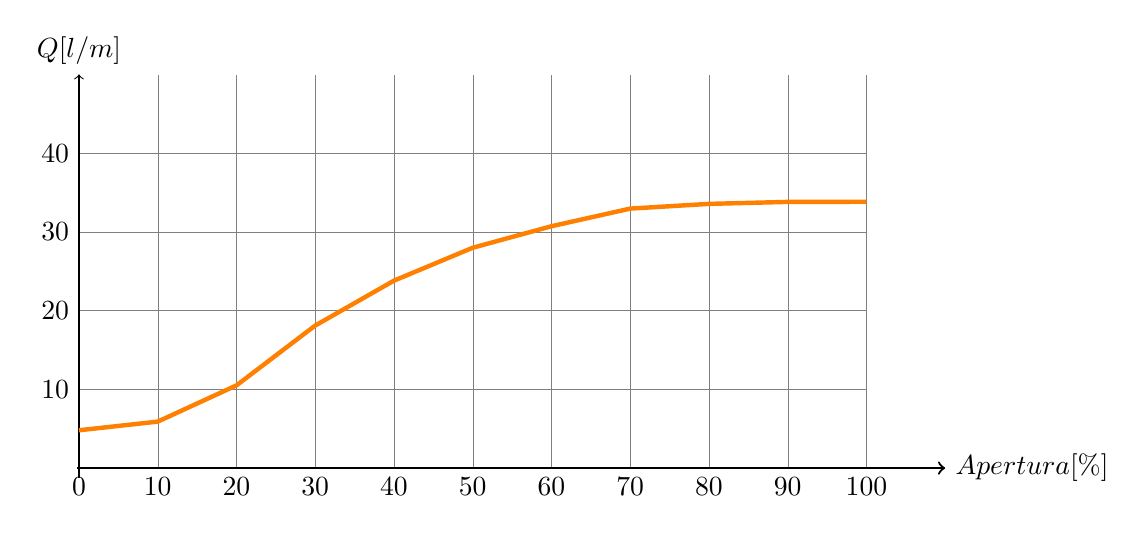
\begin{tikzpicture}[scale= 0.1, domain=0:110]
    
    \draw[ultra thin,color=gray,step=10cm] (100,49.9) grid (0.1,0.1);
    \draw[thick,->] (-0.2,0) -- (110,0) node[right,draw=none] {$Apertura [\%]$};
    \draw[->] (0,-1.2) -- (0,50) node[above,draw=none] {$Q [l/m]$};
    
    \foreach \x in {0,10,20,30,40,50,60,70,80,90,100}
    \draw (\x cm,1pt) -- (\x cm,-1pt) node[anchor=north,draw=none] {$\x$};
    \foreach \y in {10,20,30,40}
    \draw (1pt,\y cm) -- (-1pt,\y cm) node[anchor=east,draw=none] {$\y$};
    
    \draw[color = orange,ultra thick] (0,4.8) -- (10,5.9) -- (20,10.5)
    -- (30,18.1) -- (40,23.8) -- (50,27.98) -- (60,30.71)
    -- (70,32.95) -- (80,33.55) -- (90,33.8) -- (100,33.82);
   
\end{tikzpicture}
\caption{Gráfico de la válvula sin tiempo muerto.}
\label{graf:valvula}
\end{figure}

\begin{figure}\centering
  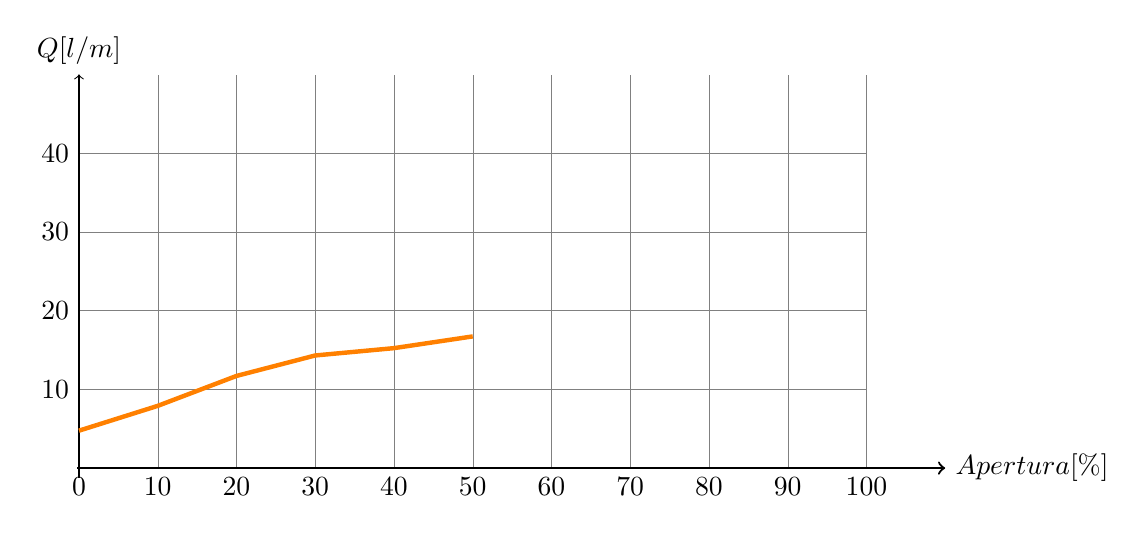
\begin{tikzpicture}[scale= 0.1, domain=0:110]
    
    \draw[ultra thin,color=gray,step=10cm] (100,49.9) grid (0.1,0.1);
    \draw[thick,->] (-0.2,0) -- (110,0) node[right,draw=none] {$Apertura [\%]$};
    \draw[->] (0,-1.2) -- (0,50) node[above,draw=none] {$Q [l/m]$};
    
    \foreach \x in {0,10,20,30,40,50,60,70,80,90,100}
    \draw (\x cm,1pt) -- (\x cm,-1pt) node[anchor=north,draw=none] {$\x$};
    \foreach \y in {10,20,30,40}
    \draw (1pt,\y cm) -- (-1pt,\y cm) node[anchor=east,draw=none] {$\y$};
    
    \draw[color = orange,ultra thick] (0,4.75) -- (10,7.9) -- (20,11.7)
    -- (30,14.3) -- (40,15.23) -- (50,16.72);
   
\end{tikzpicture}
\caption{Gráfico de la válvula con tiempo muerto.}
\label{graf:valvulatiempomuerto}
\end{figure}


\subsection{Chocked Flow}



\section{Instrumentos de Medición}
\label{sec:InstrumentosMedicion}
Para conocer el estado de la planta, es necesario tener conocimiento del
estado de numerosas variables, a saber:
\begin{itemize}
 \item \textbf{Nivel de los tanques}
 \item \textbf{Caudal en las tuberías}
 \item \textbf{Presión en las tuberías}
\end{itemize}
Debemos entonces, instalar elementos de instrumentación para poder 
medir y controlar estas variables de interés.

\subsection{DP Cell}
\label{subsec:DPCell}
 distinguimos dos celdas de presión diferencial:
  aquella que nos sirve para conocer el nivel de agua se colocó cerca del 
  tanque controlado, dado que se necesitaba conectar una de sus entradas al 
  nivel más bajo del tanque y la otra a presión atmosférica. 
  Por otro lado, la celda de presión diferencial utilizada para inferir el 
  caudal deberá conectarse a ambas secciones de la placa orificio.
  Ambas fueron fijadas a la base de madera mediante tornillos.

Se denomina \textit{DP Cell}, o celda de presión diferencial, a un sensor
que mide la diferencia de presión entre dos puntos.\todo{Una foto chabon}
En nuestro caso, entrega una corriente proporcional a la diferencia de presión 
medida en el rango de $4-20\,mA$.

La DP cell utilizada tiene las siguientes características consignadas en 
la chapa de identificación\todo{Verificar}:

\begin{table}
\centering
\begin{tabular}{|l|l|}
\hline
Marca & Yokogawa\\
Modelo & EJA 110 A\\
Tensión & $10.5\,-\,30 \, DC$\\
Output & $4-20\,mA$\\
Seguridad & MWP 160\\
\hline
\end{tabular}
\caption{Especificaciones de las celdas de presión diferencial}
\end{table}


Dos celdas serán utilizadas:
\begin{itemize}
 \item \textbf{Medición del nivel del tanque:} La celda se encuentra conectada
 al fondo del tanque controlado, y mide la presión debida al peso
 de la columna de agua en el tanque. 
 Podemos encontrar la altura del nivel en el tanque $h$ mediante la ecuación
 \begin{align}
  h &= \dfrac{P}{\gamma}
 \end{align}
donde $P$ es la presión medida por la celda, y $\gamma$ es el peso especifico
del fluído.
\item \textbf{Medición del caudal en la tubería de ida al tanque controlado:}
Se utilizará una placa orificio para generar una caída de presión debida al 
caudal (ver sección \ref{subsec:PlacaOrificio}). 
La celda deberá entonces medir la diferencia de presión antes y después
de la placa orificio.
\end{itemize}

\subsection{Placa Orificio}
\label{subsec:PlacaOrificio}
  se colocó en serie con la cañería de llenado del tanque controlado.
  Debieron instalarse además, las mangueras correspondientes de conexión 
  con la celda de presión diferencial.
  % El tablero se trata en el cap 3 :)
  %\item Tablero electrónico:
  %Estaba montado sobre la estructura una caja estanca donde se montaron todos 
  %los componentes eléctricos
  %y electrónicos.

Para medir el caudal en la tubería de ida, se decide
utilizar una placa orificio\todo{placa orif? u otra cosa?}.
En la Fig. \ref{fig:placaOrificio} se muestra un corte longitudinal de una placa
orificio.
Se observa que la placa orificio provoca una disminución del diámetro
de la cañería, con la consiguiente aceleración del fluido.
Escribiendo la ecuación de Bernoulli en 1 y 2\todo{verif. puntos}.

\begin{figure}
 \centering
 \missingfigure[figwidth=8cm]{Placa orificio}
 \caption{Corte longitudinal de una placa orificio montado en una tubería.}
 \label{fig:placaOrificio}
\end{figure}

\begin{align}
 z_1 \, \gamma + \dfrac{\rho \,v_1^2}{2} + P_1 &= z_2 \, \gamma + \dfrac{\rho \,v_2^2}{2} + P_2
\label{eq:Bernoulli}
\end{align}
donde $z_i$ y $P_i$ es la altura y presión en el punto $i$ y $\rho$ es 
la densidad del fluido. 
Considerando que la altura en ambos puntos es la misma, la ecuación
\eqref{eq:Bernoulli} puede reescribirse como
\begin{align}
 v_2^2 - v_1^2 &= 2\,g\,h_p
 \label{eq:Bernoulli2}
\end{align}
donde $h_p$ es la diferencia de presión entre 1 y 2, expresada como 
altura de la columna fluida
\begin{align}
 h_p &= \dfrac{P_1}{\gamma}-\dfrac{P_2}{\gamma}
\end{align}
La ecuación de continuidad, para fluidos incompresibles se escribe
\begin{align}
 A_1\,v_1 &= A_2\,v_2 \\
 v_2 &= \dfrac{A_1}{A_2} v_1 \\
 v_2 &= \dfrac{D_1^2}{D_2^2} v_1
 \label{eq:velRef}
\end{align}
y reemplazando \eqref{eq:velRef} en \eqref{eq:Bernoulli2} obtenemos
\begin{align}
 2 \, g \, h_p &= v_2^2 \left( 1 - \dfrac{D_1^4}{D_2^4} \right)\\
 \beta &= \dfrac{D_1}{D_2}\\
 v_2 &= \sqrt{\dfrac{2 \, g \, h_f}{1-\beta^4}} 
\end{align}
finalmente, el caudal se obtiene multiplicando la velocidad $v_2$ por el
área $A_2$.
Además, se agrega un coeficiente $C_v$ debido al fenómeno de vena contracta:
\begin{align}
 Q &= \dfrac{C_v \, A_2}{\sqrt{1-\beta^4}}\, \sqrt{2 \, g \, h_f}
 \label{eq:placaOrif1}
\end{align}
El coeficiente $C_v$ depende del número de Reynolds $Re$ \cite{bib:Mataix, bib:ApuntesPuglesiPlacaOrif}
\begin{align}
Re &= \dfrac{D\,v}{\nu}
\end{align}
donde $v$ es la velocidad en la placa orificio, $D$ es el diámetro y ${\nu}$
es la viscosidad cinemática del fluido\footnote{Para el agua, nuestro fluido de trabajo
$\nu = 1,003\,10^{-6} \frac{m^2}{s}$.}

La ecuación \eqref{eq:placaOrif1} puede ser reescrita de una forma más sencilla
mediante una nueva variable adimensional $C_q$
\begin{align}
 C_q &= \dfrac{C_v}{\sqrt{1-\beta^4}}
\end{align}
$C_q$ depende tanto del número de Reynolds como de la razón de los diámetros $\beta$, 
y su valor numérico puede ser encontrado en tablas y ábacos en la bibliografía \cite{bib:Mataix},
\todo{Lo encontramos así, o de otra manera experimental al cq?}

Finalmente, la ecuación a aplicar en el autómata para medir el caudal es
\begin{align}
 Q &= C_q\,A_2\, \sqrt{2\,g\,h_f}
\end{align}
donde se observa que el caudal $Q$ es proporcional a $\sqrt{h_f}$, que puede
ser encontrada utilizando un DP cell (ver sección \ref{subsec:DPCell}).

\subsection{Manómetros}
\label{subsec:Manometros}

\begin{figure}[ht]
 \centering
 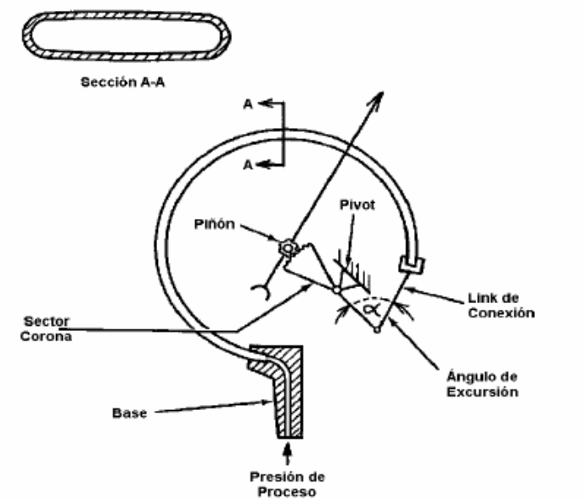
\includegraphics[width=.7\textwidth]{Cap2-DisenoEnsamblado/images/manomBourdon.png}
 \caption{Manómetro de Bourdon, extraído de \cite{bib:ApuntesPuglesiPlacaOrif}}
 \label{fig:manometroBourdon}
\end{figure}

Para conocer los valores de presión en ambas cañerías
(referirse al \gls{pyid}, sección \ref{sec:p&id}),
se instalaron manómetros comunes, de tipo Bourdon\todo{Escala de los manoms?}. 
Un ejemplo de estos manómetros se muestra en la Fig. \ref{fig:manometroBourdon},
donde se observa que un incremento de la presión produce una deformación 
del \emph{tubo de Bourdon}, reflejado en la aguja indicadora.
El manómetro de Bourdon permite obtener una medición visual de la
presión relativa, del punto donde se encuentra instalado.

Durante el montaje, se presentó el problema que uno de los manómetros
no entregaba una medición definida, sino que oscilaba alrededor de un
valor medio (imposibilitando la lectura directa)\todo{por qué pasa esto?}.
Este problema fue solucionado instalando un \textbf{manómetro con glicerina},
donde el mecanismo del manómetro se encuentra sumergido en un baño de glicerina.
Debido a la viscosidad del fluido, las vibraciones quedan amortiguadas
y el manómetro refleja el valor medio de la presión.
